
\clearpage
\section{Configuration}

\begin{wrapfigure}[14]{l}{6.5cm}   % [x] Wie manche Zeile soll sich um die Grafik "brechen"
  \vspace{-35pt}      % Grundwert war 20; mit 30 schön oben beim Text ausgerichtet
  \begin{center}
    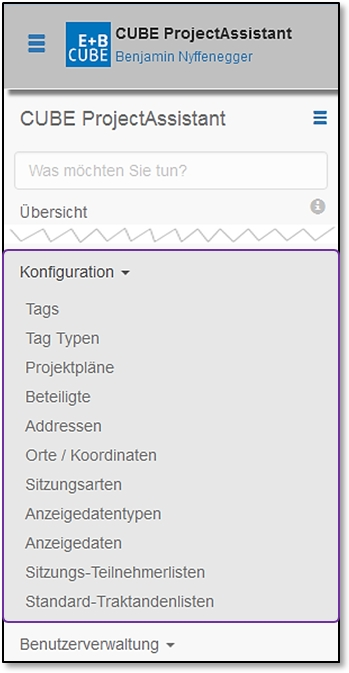
\includegraphics[width=1\linewidth]{../chapters/13_Konfigurationen/pictures/13_Menu_Konfiguration.jpg}
  \end{center}
  \vspace{-20pt}
  \caption{Configuring CUBE PA}
  \vspace{-10pt}
\end{wrapfigure}

Configuration is usually carried out by the administrator or a so-called power user who has been trained specially for this purpose. Accordingly, this chapter does not go through the configuration process in detail. In case of doubt it is recommended to contact CUBE PA support for open questions or uncertainties (see chapter \ref{bkm:Ref443502661}).

\vspace{\baselineskip}

In the menu on the left, select the 'Configuration' menu item. The sub-items that appear are briefly presented below.

\vspace{1.5cm} 

For users who do not have the required access authorizations, these points will not be displayed.\\

\vspace{3.5cm}  

\textbf{Overview of the configuration possibilities:}

\vspace{\baselineskip}

\begin{itemize}
\item
\textbf{Tags}: Tags can be entered and sorted into 'tag types'. Tags are used in document management for example in order to designate documents by theme and be able to find them more easily. 
The 'Projects / Subprojects' tags are used in many places in CUBE PA (e.g. Meeting management, Procurement function).
\item
\textbf{Tag types}: Tag types (categories), in which individual tags can later be sorted, 
can be defined.
\item
\textbf{Project plans}: Several project plans (e.g. detailed scheduling program) can be created. The project plans can be selected and imported separately using the 'Import' (then 'Project plan data') function.
\item
\textbf{Participants}: Participants can be created in order to be used for various purposes in CUBE PA. Participants are mostly companies, committees or other organizational units. Depending on their function in the project, they can be marked as a 'company', 'client', 'contractor', 'committee', etc. The marking affects where in CUBE PA the corresponding participants appear in the selection boxes.
\item
\textbf{Addresses}: Addresses, which can be used as meeting venues or location of meeting minutes, can be created.
\item
\textbf{Location / Coordinates}: These entries refer to project-related 'locations', e.g. level crossings, train stations, etc., which can be linked to Google Maps. These predefined Locations / Coordinates facilitate the assignment of coordinates to documents under document management. Their use is however optional. Coordinates which have not been previously defined can also be assigned to documents.
\item
\textbf{Meeting types}: The different meeting types and responsibilities can be managed. In the current version of CUBE PA, the management of access rights for the meetings takes place exclusively under the user management.
\item
\textbf{Data resource types and data resources}: Important information documents, which should be accessible for the users with a few clicks, can be stored. This is done via configurable additional entries in the menu, or so-called data resource types. For each data resource type, the menu category in which the entry should appear can be specified (e.g. in Meeting management or Quality management). The actual documents are called data resources. 
Several data resources can be sorted under the same resource data type. It is also possible to specify which person is to be responsible for a particular data resource. It is recommended to only use this function sparingly, otherwise the main menu could be overloaded. The function can for example be used for displaying a complete scheduling program if it's only available in the form of an Excel file and not in the form of an MS Project file.
\item
\textbf{Meeting participant lists}: Optional meeting participant lists can be put together for meetings. It can also be defined whether the selected participants are on the distribution list or not. The lists can then be selected during the creation of meeting invitations.
\item
\textbf{Default agenda item lists}: Constantly recurring agenda item lists can be predefined under this function and later selected during the creation of a meeting.
\end{itemize}

\vspace{\baselineskip}

The various input masks of the above described configuration points are briefly documented below. For further detailed or other information please contact the CUBE PA support: {\color{red} cube.support@emchberger.ch}

\subsection{Tags}

New tags can be created, viewed or edited here.

\begin{figure}[H]
\center{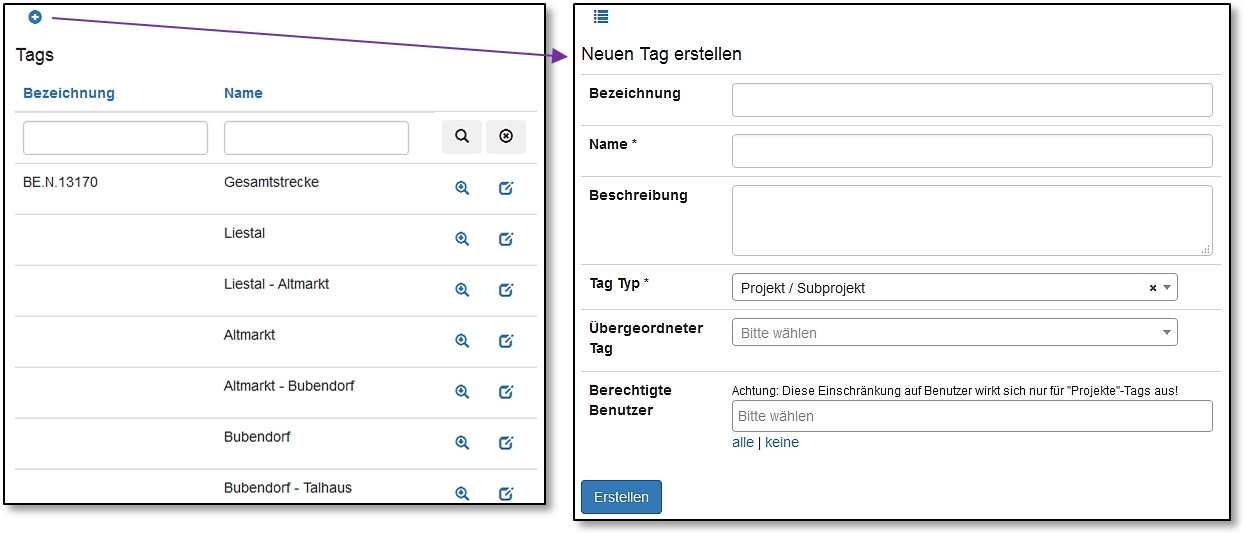
\includegraphics[width=1\linewidth]{../chapters/13_Konfigurationen/pictures/13-1_TagsHinzufuegen.jpg}}
\caption{Creating new tags}
% \label{fig:speciation}
\end{figure}

The 'Identifier' is momentarily only used for the Project / Subproject tags. A project number can be entered here.

\vspace{\baselineskip}

The 'Name' (mandatory field) is used throughout CUBE PA for the corresponding tag.

\vspace{\baselineskip}

Tags must be assigned to a tag type (see chapter \ref{bkm:Ref444100222}).

\vspace{\baselineskip}

It is possible to set up a tag hierarchy. To do so, the 'parent tag' field should be filled for a child tag. Several children tags can be assigned to the same parent tag.

\vspace{\baselineskip}

In a later version of CUBE PA, it will be possible to include children tags in the tag filtering and search functions. In the current version of CUBE PA, the tag hierarchy is still limited.

\vspace{\baselineskip}

Note that the selection of authorized users is only active for 'Project' tags (see note).

\subsection{Tag types}
\label{bkm:Ref444100222}
Since tags are a very universal tool in CUBE PA, it is possible to define different tag categories called tag types.\newline

This makes tagging documents according to various criteria possible. Such examples include the document type or the subject area. The 'Project / Subproject' category is also stored as a tag type and is used when the 'is project' box is checked. This ensures that the tags of this category can be selected wherever the assignment to a subporject is desired (e.g. in meetings or procurements). \newline

Tag types that are to be used for the categorization of documents can be used when the 'is document tag type' box is checked. The display sequence of the tag types can be set by entering a number into the 'Position' field. The sequence is ascending.

\begin{figure}[H]
\center{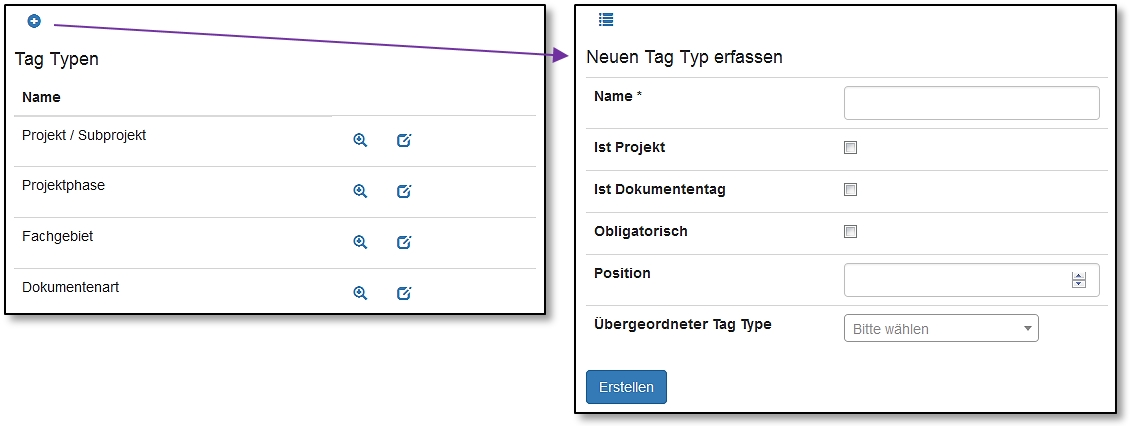
\includegraphics[width=1\linewidth]{../chapters/13_Konfigurationen/pictures/13-2_TagTypenHinzufuegen.jpg}}
\caption{Creating a new tag type}
% \label{fig:speciation}
\end{figure}\pagebreak

\subsection{Project plans}

Several project plans (e.g. detailed scheduling program, scheduling program for subprojects) can be created, for which separate entries can be imported using the 'Import' (then 'Project plan data') function.

\begin{figure}[H]
\center{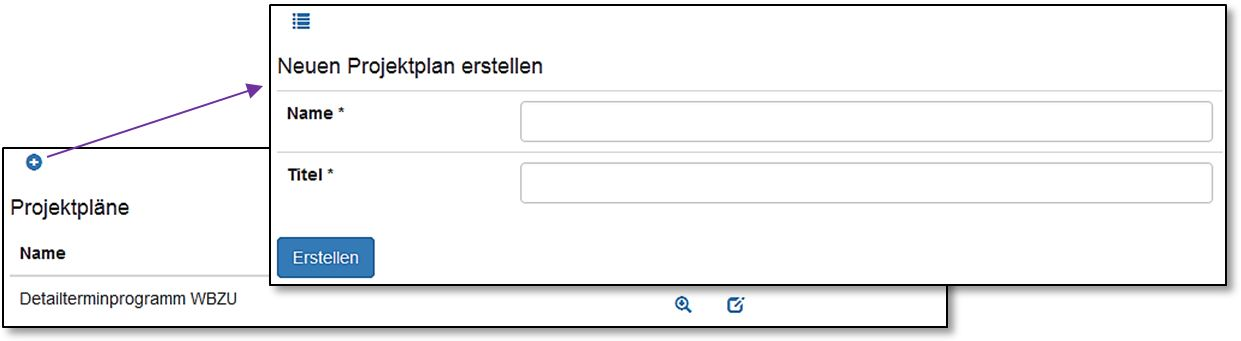
\includegraphics[width=1\linewidth]{133_ProjektplaeneHinzufuegen.jpg}}
\caption{Creating a new project plan}
% \label{fig:speciation}
\end{figure}

All created project plans are listed here. They can be viewed or modified in the detailed view. New entries can also be created under this configuration point.

\subsection{Participants}

\begin{wrapfigure}[11]{r}{6cm}
\vspace{-25pt}
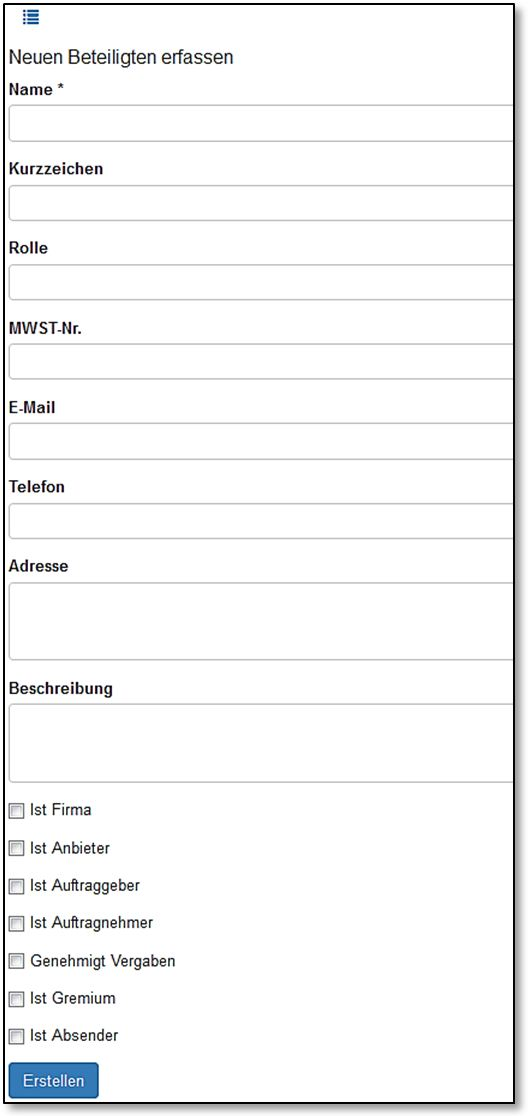
\includegraphics[height=150mm]{134_BeteiligteHinzufuegen.jpg}
% \caption{Status ändern}
\end{wrapfigure}

Participants involved in a project can be entered here and then be assigned various 'roles'.

\begin{center}
\hspace{-15pt}   
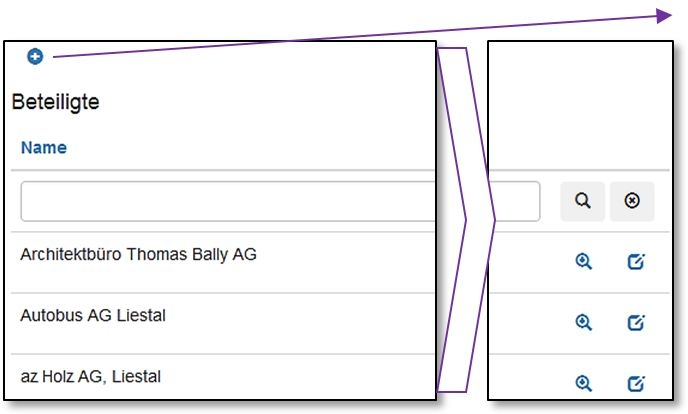
\includegraphics[width=.9\linewidth]{../chapters/13_Konfigurationen/pictures/13-4_Beteiligte.jpg}
\end{center}

The 'Roles' field is a free text field in which the role of a participant within a project can be defined.

\vspace{\baselineskip}

The below check boxes 'is company', 'is client' etc. enable the participants to be referenced and available for selection in CUBE PA areas. For example, if '[x] is company' is selected, the participant will be available for selection in the 'company' selection / dropdown field.

\vspace{\baselineskip}
\vspace{\baselineskip}
\vspace{\baselineskip}

% -->>> Wenn \clearpage löschen > Achtung Formatierung zu vorhergehendem Bild beachten -> allenfalls \clearpage bestehen lassen
% \clearpage
\subsection{Addresses}

Addresses are generally meeting rooms. Locations (without a meeting room function) can also be entered. The 'is meeting room' check-box should accordingly be checked or left blank when creating an address. 

\begin{figure}[H]
\center{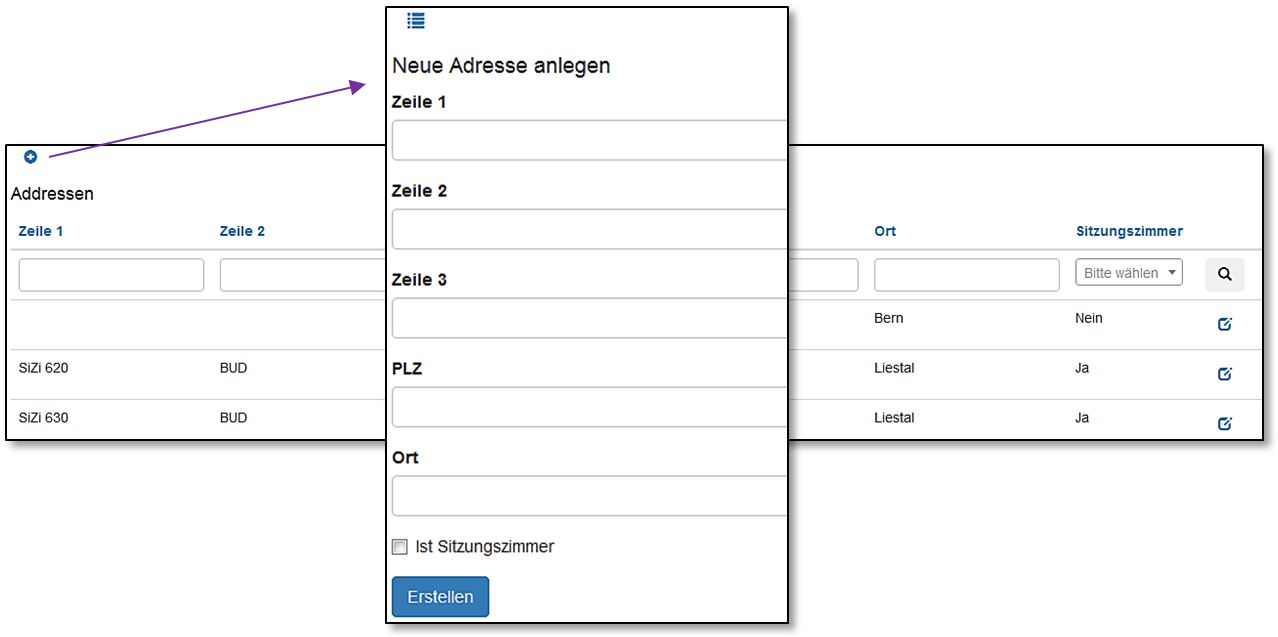
\includegraphics[width=1\linewidth]{135_AdresseHinzufuegen.jpg}}
\caption{Creating a new address}
% \label{fig:speciation}
\end{figure}

\subsection{Locations / Coordinates}

These entries refer to project-related 'locations', e.g. level crossings, train stations etc., that can be linked to Google Maps. Clicking on the pin displays the labeled position in Google Maps.

\begin{figure}[H]
\center{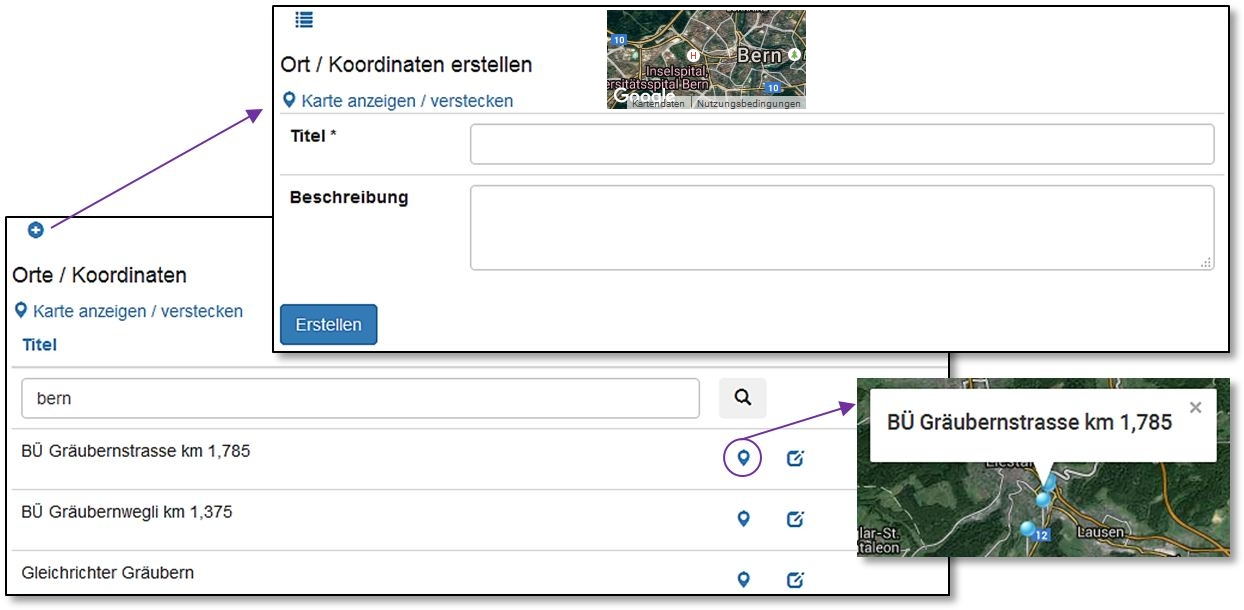
\includegraphics[width=1\linewidth]{../chapters/13_Konfigurationen/pictures/13-6_KoordinatenHinzufuegen.jpg}}
\caption{Creating locations / coordinates}
% \label{fig:speciation}
\end{figure}

\clearpage
\subsection{Meeting types}

The different meeting types and the accordingly authorized users are created here.

\vspace{\baselineskip}


The 'Chairman' and 'Deputy' of a meeting can be predefined and if necessary 
later modified.

\begin{figure}[H]
\center{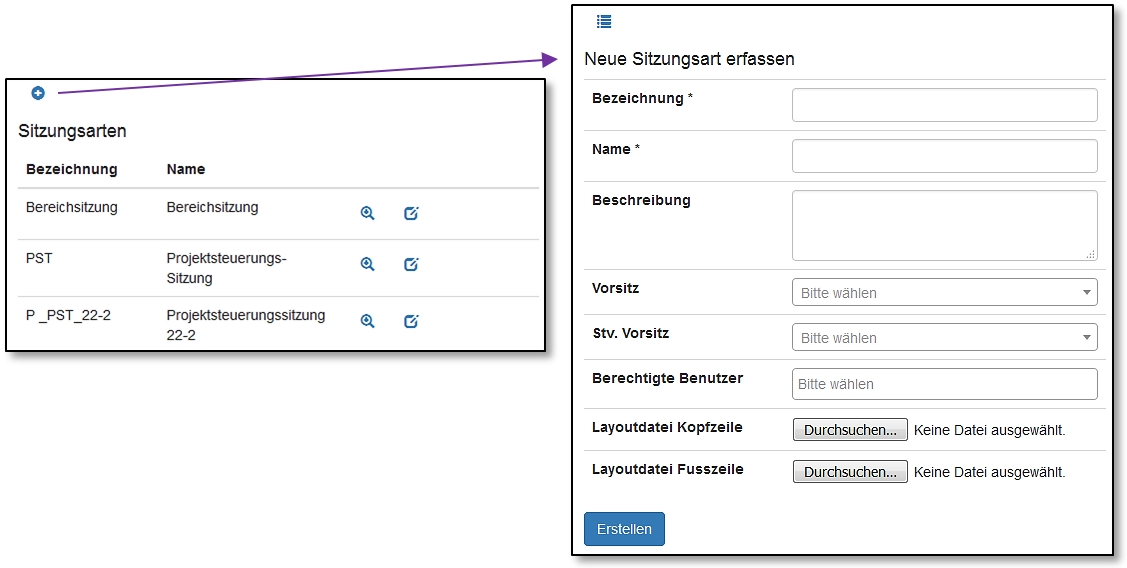
\includegraphics[width=1\linewidth]{../chapters/13_Konfigurationen/pictures/13-7_SitzungsartHinzufuegen.jpg}}
\caption{Creating a new meeting type}
% \label{fig:speciation}
\end{figure}

\subsection{Data resource types and data resources}

Important information documents, which should be accessible for the users with a few clicks, can be stored. This is done via configurable additional entries in the menu, or so-called data resource types. For each data resource type, the menu category in which the entry should appear can be specified (e.g. in Meeting management or Quality management). The actual documents are called data resources. Several data resources can be sorted under the same resource data type. It is also possible to specify which person is to be responsible for a particular data resource. It is recommended to only use this function sparingly, otherwise the main menu could be overloaded. The function can for example be used for displaying a complete scheduling program if it's only available in the form of an Excel file and not in the form of an MS Project file.

\vspace{\baselineskip}

The name of a data resource type is to be kept as concise and short as possible. According to the entry (name), this will be displayed in the menu under the selected category. For this reason, several words or a sentence are to be avoided.

\begin{figure}[H]
\center{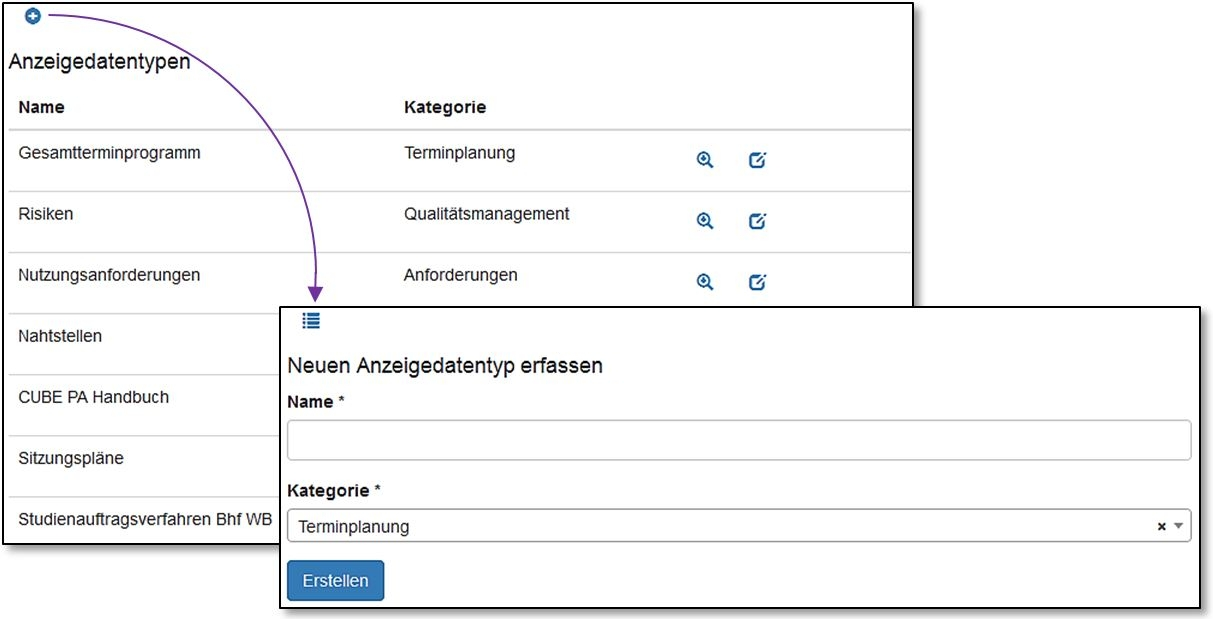
\includegraphics[width=1\linewidth]{138_AnzeigetypenErfassen.jpg}}
\caption{Creating new data resource types}
% \label{fig:speciation}
\end{figure}

\begin{figure}[H]
\center{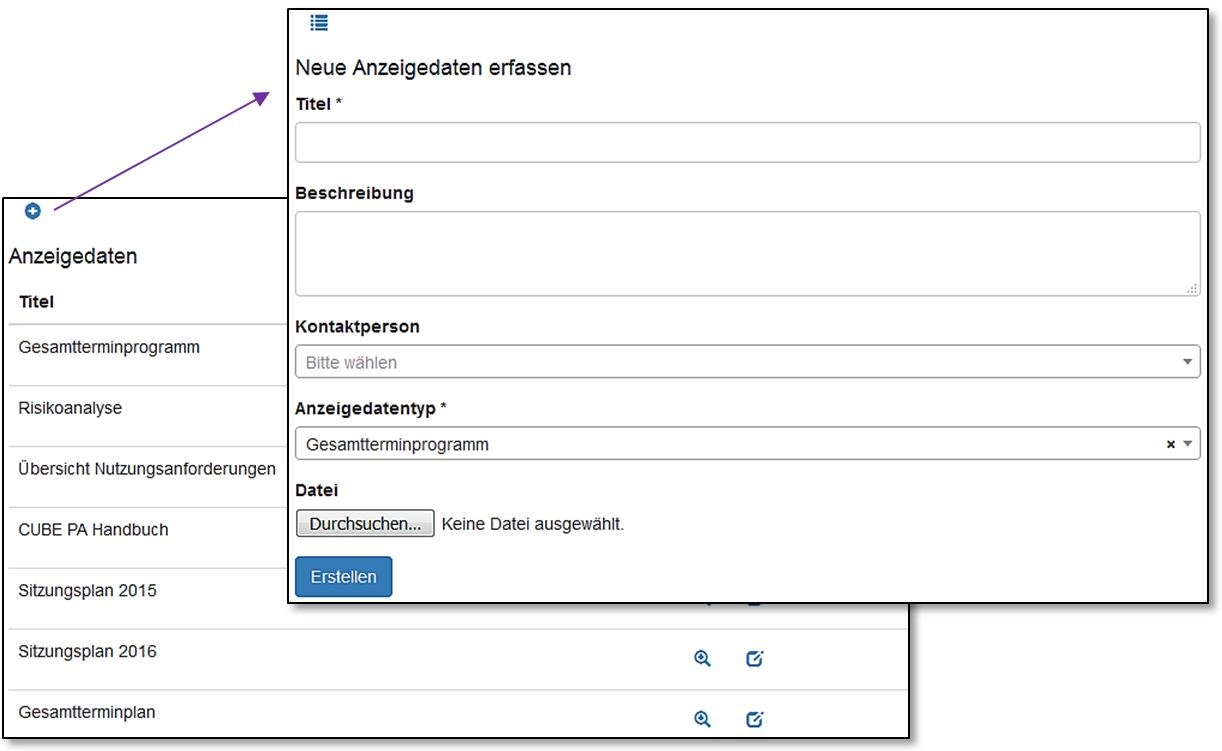
\includegraphics[width=1\linewidth]{138_AnzeigedatenErfassen.jpg}}
\caption{Creating new data resources}
% \label{fig:speciation}
\end{figure}

% \small{Übersicht und Eingabemöglichkeiten für die Anzeigedatentypen und Anzeigedaten.}

\subsection{Meeting participant lists}

Any number of meeting participant lists can be put together for meetings. It can also be defined whether the selected participants are on the distribution list or not.

\begin{figure}[H]
\center{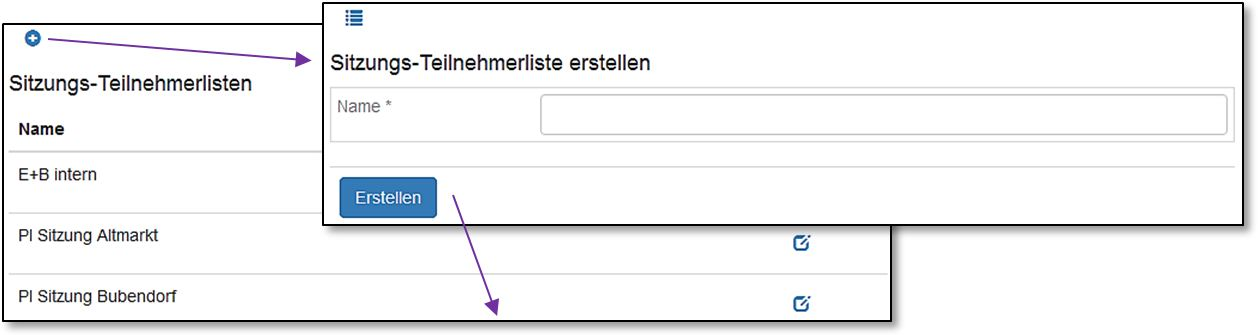
\includegraphics[width=1\linewidth]{139_SitzungsteilnehmerlistenErstellen.jpg}}
% \caption{Sitzungs-Teilnehmerlisten erstellen}
% \label{fig:speciation}
\end{figure}

\begin{figure}[H]
\vspace{-25pt}
\center{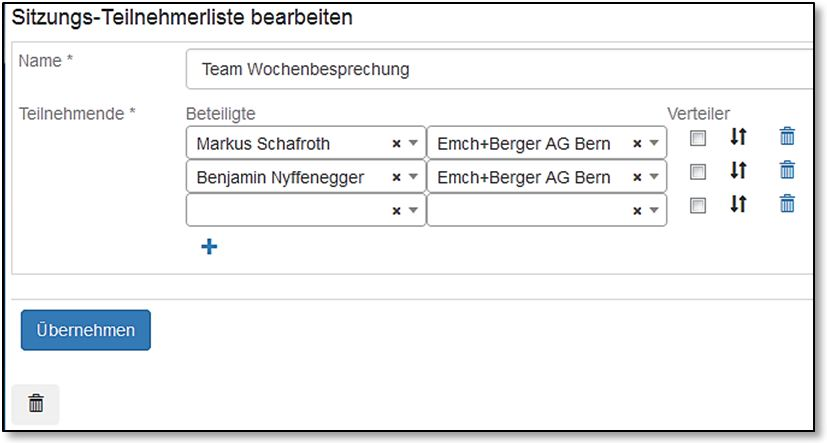
\includegraphics[width=0.55\linewidth]{139_SitzungsteilnehmerlistenBearbeiten.jpg}}
\caption{Creating and editing meeting participant lists}
% \label{fig:speciation}
\end{figure}

Only after clicking 'Create' is it possible to add members to a new list. Members can be moved in the list to change their order or can be removed from the list. A meeting participant list can be deleted at the bottom of the window.

\clearpage
\subsection{Default agenda item lists}

Constantly recurring agenda item lists can be predefined under this function and later selected during the creation of a meeting.

\begin{figure}[H]
\center{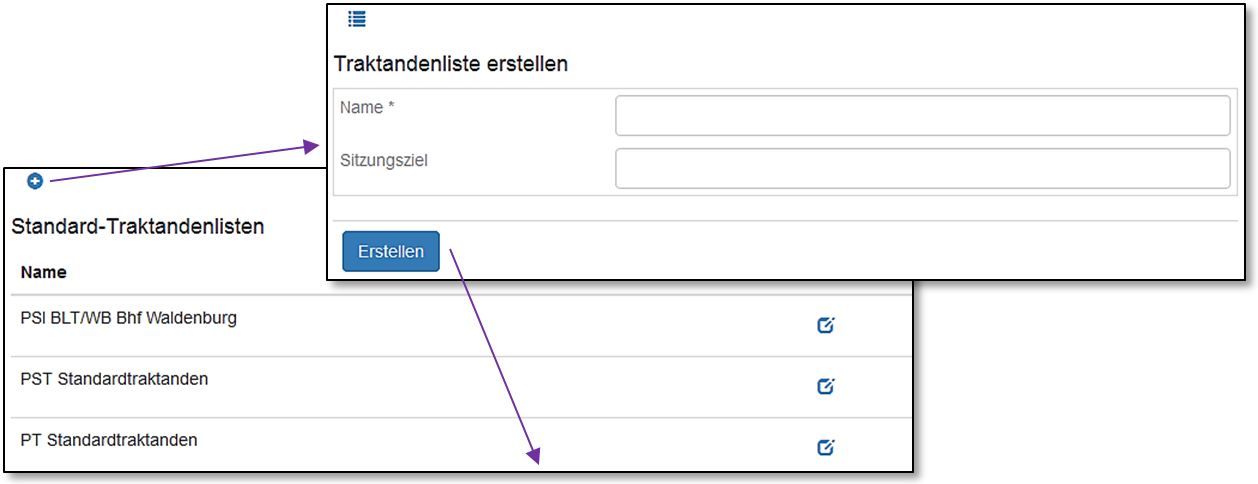
\includegraphics[width=1\linewidth]{1310_TraktandenlistenErstellen.jpg}}
\caption{Creating agenda item lists}
% \label{fig:speciation}
\end{figure}

\begin{wrapfigure}[12]{r}{9cm}
\vspace{-15pt}
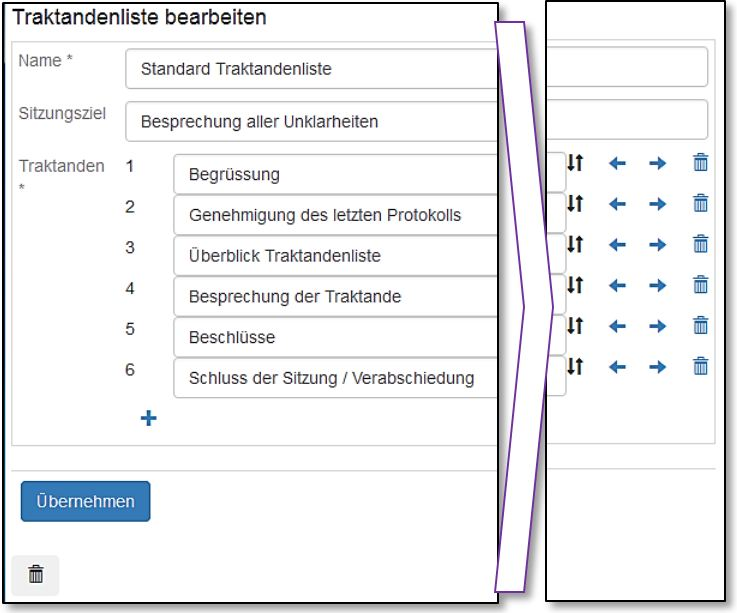
\includegraphics[height=80mm]{1310_TraktandenlistenBearbeiten.jpg}
% \caption{Status ändern}
\end{wrapfigure}

Only after 'creating' a new agenda item list does it become possible to add or edit agenda items. New agenda items can be moved to change the order or the outline (1, 2, 3 or 2, 2.1, 3 etc.). You can delete individual agenda items as well as whole agenda item lists.
